\documentclass[12pt,a4paper]{article}
\usepackage[utf8]{vietnam}
\usepackage{amsmath,amssymb}
\usepackage{tabularx}
\usepackage{tikz}
\usepackage{xcolor}
\usepackage[top=0.6cm, bottom=0.6cm, left=0.6cm, right=0.6cm]{geometry}
\usepackage[dethi]{ex_test}

\SAOPTN{widthSA=2.6,heightSA=0.62}
\setlength{\parskip}{0pt}

% Dong ke cham mo chuan viet tay
\newcommand{\dongke}[1]{%
  \begingroup%
  \setlength{\parskip}{0pt}%
  \baselineskip=18.5pt%
  \vspace{1.0mm}%
  \foreach \i in {1,...,#1}{%
    \noindent{\color{gray!60}\dotfill}\par%
  }%
  \vspace{0.6mm}%
  \endgroup%
}

% Khu vuc bai lam chia 2 cot co vach ngan mo o giua
\newcommand{\dongkeHaiCot}[1]{%
  \par\vspace{0.5mm}%
  \noindent%
  \begin{minipage}[t]{0.485\linewidth}%
    \dongke{#1}%
  \end{minipage}%
  \hfill%
  {\color{gray!60}\vrule}%
  \hfill%
  \begin{minipage}[t]{0.485\linewidth}%
    \dongke{#1}%
  \end{minipage}%
}

% Dinh nghia o bai tap tu luan trong bang
\newcommand{\oBaiTap}[3][5]{%
  \vspace{1.0mm}%
  \noindent\textbf{#2} #3\par%
  \dongke{#1}%
}

\begin{document}
\pagestyle{empty}
% =============================================================================
% ========================= TOAN 8 TUAN 09 BUOI 02 - MA DE 101 =================
% ========================= TRANG 1/2 ==========================================
% =============================================================================
\noindent
\begin{tabularx}{\linewidth}{|X|c|}
\hline
\textbf{PHIẾU KIỂM TRA ĐỊNH KỲ TOÁN 8 - TUẦN 09 - BUỔI 02} & \textbf{Mã đề: 101 - Trang 1/2} \\
\hline
\end{tabularx}

\vspace{1.2mm}

\noindent
\begin{tabularx}{\linewidth}{|p{3.2cm}|X|}
\hline
\centering\textbf{ĐIỂM SỐ} & \centering\textbf{LỜI NHẬN XÉT CỦA THẦY CÔ} \tabularnewline
\hline
\rule{0pt}{1.8cm} & \tabularnewline
\hline
\end{tabularx}

\vspace{1.4mm}
\noindent\textbf{Câu 1 (0,25 điểm).} Bậc của đơn thức $A = 5x^4 y^2 z^2$ là: \shortans{8}\par\vspace{2.3mm}
\noindent\textbf{Câu 2 (0,25 điểm).} Bậc của đa thức $P = 5x^2 y^2 - 3x^3 - 5x^2 y^2 + 2x^3 + 8$ là: \shortans{3}\par\vspace{2.3mm}
\noindent\textbf{Câu 3 (0,25 điểm).} Giá trị của $M = 3x^2 y - 2xy$ tại $x=1, y=-3$ bằng: \shortans{-3}\par\vspace{2.3mm}
\noindent\textbf{Câu 4 (0,25 điểm).} Cho khai triển $(x-4)(x+4) = x^2 - a$. Giá trị của $a$ là: \shortans{16}\par\vspace{2.3mm}
\noindent\textbf{Câu 5 (0,25 điểm).} Tính nhanh giá trị biểu thức $101^2 - 1 = $: \shortans{10\,200}\par\vspace{2.3mm}
\noindent\textbf{Câu 6 (0,25 điểm).} Phân tích đa thức thành bình phương: $x^2 - 8x + 16 = $: \shortans{(x - 4)^2}\par\vspace{2.3mm}
\noindent\textbf{Câu 7 (0,25 điểm).} Kết quả phép chia $(15x^3 y^2 - 9x^2 y) : (3x^2 y)$ là: \shortans{5xy - 3}\par\vspace{2.3mm}
\noindent\textbf{Câu 8 (0,25 điểm).} Hình thoi có chu vi $28\text{ cm}$. Độ dài mỗi cạnh của hình thoi là: \shortans{7\text{ cm}}\par\vspace{2.3mm}
\noindent\textbf{Câu 9 (0,25 điểm).} Hình chữ nhật có hai đường chéo vuông góc là hình gì?: \shortans{Hình vuông}\par\vspace{2.3mm}
\noindent\textbf{Câu 10 (0,25 điểm).} Hình thoi có độ dài hai đường chéo là $6\text{ m}$ và $8\text{ m}$. Diện tích hình thoi là: \shortans{24\text{ m}^2}\par\vspace{2.3mm}
\vspace{0.2mm}
\noindent\textbf{Câu 11 (3,0 điểm). Thực hiện phép tính và phân tích đa thức thành nhân tử:}
\vspace{0.8mm}

\noindent
\begin{tabularx}{\linewidth}{|X|X|}
\hline
\oBaiTap[6]{a) (0,5 điểm)}{$3x(2x^2 - 5x + 3)$} & 
\oBaiTap[6]{b) (0,5 điểm)}{$(2x - 1)(x + 4) - 2x^2$} \\
\hline
\oBaiTap[6]{c) (0,5 điểm)}{$(2x - 3)^2 + (2x + 3)^2$} & 
\oBaiTap[6]{d) (0,5 điểm)}{$x^2 - xy + 3x - 3y$} \\
\hline
\oBaiTap[6]{e) (0,5 điểm)}{$x^2 - 4y^2 + 2x + 1$} & 
\oBaiTap[6]{f) (0,5 điểm)}{$x^2 - 5x + 6$} \\
\hline
\end{tabularx}

\newpage
% =============================================================================
% ========================= TOAN 8 TUAN 09 BUOI 02 - MA DE 101 =================
% ========================= TRANG 2/2 ==========================================
% =============================================================================
\noindent
\begin{tabularx}{\linewidth}{|X|c|}
\hline
\textbf{TOÁN 8 - TUẦN 09 - BUỔI 02} & \textbf{Mã đề: 101 - Trang 2/2} \\
\hline
\end{tabularx}

\vspace{1.4mm}

\noindent\textbf{Câu 12 (2,0 điểm). Tìm số thực $x$, biết:}
\vspace{0.8mm}

\noindent
\begin{tabularx}{\linewidth}{|X|X|}
\hline
\oBaiTap[5]{a) (0,5 điểm)}{$4x(x - 3) - 4x^2 = -24$} & 
\oBaiTap[5]{b) (0,5 điểm)}{$x(x - 6) + 4(x - 6) = 0$} \\
\hline
\oBaiTap[5]{c) (0,5 điểm)}{$(x - 2)^2 - 25 = 0$} & 
\oBaiTap[5]{d) (0,5 điểm)}{$(2x + 3)^2 = 49$} \\
\hline
\end{tabularx}

\vspace{1.4mm}

\noindent
\begin{tabularx}{\linewidth}{|X|}
\hline
\vspace{0.5mm}
\begin{minipage}[t]{0.64\linewidth}
\vspace{0pt}
\textbf{Câu 13 (2,0 điểm).} Cho tam giác $ABC$ cân tại $A$, đường trung tuyến $AM$. Gọi $I$ là trung điểm của $AC$. Lấy điểm $K$ đối xứng với $M$ qua $I$.\par\vspace{0.4mm}
\textbf{a)} (1,0 điểm) Chứng minh tứ giác $AMCK$ là hình chữ nhật.\par\vspace{0.4mm}
\textbf{b)} (1,0 điểm) Chứng minh tứ giác $ABMK$ là hình bình hành. Suy ra $AK \parallel BC$ và $AK = MC$.
\end{minipage}\hfill
\begin{minipage}[t]{0.34\linewidth}
\vspace{0pt}\centering
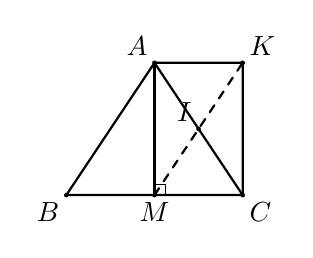
\begin{tikzpicture}[scale=0.70, >=stealth, line join=round, line cap=round]
  \coordinate (B) at (-1.6, 0);
  \coordinate (C) at (1.6, 0);
  \coordinate (M) at (0, 0);
  \coordinate (A) at (0, 2.4);
  \coordinate (I) at (0.8, 1.2);
  \coordinate (K) at (1.6, 2.4);
  \draw[thick] (B) -- (A) -- (K) -- (C) -- cycle;
  \draw[thick] (A) -- (M);
  \draw[thick] (A) -- (C);
  \draw[thick, dashed] (M) -- (K);
  \draw (0, 0.2) -- (0.2, 0.2) -- (0.2, 0);
  \fill (A) circle (1.2pt) node[above left=-1pt] {$A$};
  \fill (B) circle (1.2pt) node[below left=-1pt] {$B$};
  \fill (C) circle (1.2pt) node[below right=-1pt] {$C$};
  \fill (M) circle (1.2pt) node[below=-1pt] {$M$};
  \fill (I) circle (1.2pt) node[above left=-1pt] {$I$};
  \fill (K) circle (1.2pt) node[above right=-1pt] {$K$};
\end{tikzpicture}
\end{minipage}\par
\vspace{0.4mm}
\noindent\textit{Bài giải:}\dongkeHaiCot{11}
\\ \hline
\end{tabularx}

\vspace{1.4mm}

\noindent
\begin{tabularx}{\linewidth}{|X|}
\hline
\vspace{0.5mm}
\textbf{Câu 14 (0,5 điểm).} Tìm giá trị lớn nhất của biểu thức: $B = -x^2 + 6x + 2015$.\par
\vspace{0.4mm}
\noindent\textit{Bài giải:}\dongkeHaiCot{7}
\\ \hline
\end{tabularx}

\newpage
% =============================================================================
% ========================= TOAN 8 TUAN 09 BUOI 02 - MA DE 102 =================
% ========================= TRANG 1/2 ==========================================
% =============================================================================
\noindent
\begin{tabularx}{\linewidth}{|X|c|}
\hline
\textbf{PHIẾU KIỂM TRA ĐỊNH KỲ TOÁN 8 - TUẦN 09 - BUỔI 02} & \textbf{Mã đề: 102 - Trang 1/2} \\
\hline
\end{tabularx}

\vspace{1.2mm}

\noindent
\begin{tabularx}{\linewidth}{|p{3.2cm}|X|}
\hline
\centering\textbf{ĐIỂM SỐ} & \centering\textbf{LỜI NHẬN XÉT CỦA THẦY CÔ} \tabularnewline
\hline
\rule{0pt}{1.8cm} & \tabularnewline
\hline
\end{tabularx}

\vspace{1.4mm}
\noindent\textbf{Câu 1 (0,25 điểm).} Bậc của đơn thức $B = -3x^3 y^3 z^3$ là: \shortans{9}\par\vspace{2.3mm}
\noindent\textbf{Câu 2 (0,25 điểm).} Bậc của đa thức $Q = 4x^3 y - 2xy^2 - 4x^3 y + 5xy^2 - 1$ là: \shortans{3}\par\vspace{2.3mm}
\noindent\textbf{Câu 3 (0,25 điểm).} Giá trị của $N = 2x^2 y - 4xy$ tại $x=1, y=-2$ bằng: \shortans{4}\par\vspace{2.3mm}
\noindent\textbf{Câu 4 (0,25 điểm).} Cho khai triển $(x-5)(x+5) = x^2 - b$. Giá trị của $b$ là: \shortans{25}\par\vspace{2.3mm}
\noindent\textbf{Câu 5 (0,25 điểm).} Tính nhanh giá trị biểu thức $201^2 - 1 = $: \shortans{40\,400}\par\vspace{2.3mm}
\noindent\textbf{Câu 6 (0,25 điểm).} Phân tích đa thức thành bình phương: $x^2 - 10x + 25 = $: \shortans{(x - 5)^2}\par\vspace{2.3mm}
\noindent\textbf{Câu 7 (0,25 điểm).} Kết quả phép chia $(18x^4 y^3 - 12x^3 y^2) : (6x^3 y^2)$ là: \shortans{3xy - 2}\par\vspace{2.3mm}
\noindent\textbf{Câu 8 (0,25 điểm).} Hình thoi có chu vi $36\text{ cm}$. Độ dài mỗi cạnh của hình thoi là: \shortans{9\text{ cm}}\par\vspace{2.3mm}
\noindent\textbf{Câu 9 (0,25 điểm).} Hình chữ nhật có hai cạnh kề bằng nhau là hình gì?: \shortans{Hình vuông}\par\vspace{2.3mm}
\noindent\textbf{Câu 10 (0,25 điểm).} Hình thoi có độ dài hai đường chéo là $10\text{ m}$ và $12\text{ m}$. Diện tích hình thoi là: \shortans{60\text{ m}^2}\par\vspace{2.3mm}
\vspace{0.2mm}
\noindent\textbf{Câu 11 (3,0 điểm). Thực hiện phép tính và phân tích đa thức thành nhân tử:}
\vspace{0.8mm}

\noindent
\begin{tabularx}{\linewidth}{|X|X|}
\hline
\oBaiTap[6]{a) (0,5 điểm)}{$2x(3x^2 - 4x + 5)$} & 
\oBaiTap[6]{b) (0,5 điểm)}{$(3x - 1)(x + 2) - 3x^2$} \\
\hline
\oBaiTap[6]{c) (0,5 điểm)}{$(3x - 2)^2 + (3x + 2)^2$} & 
\oBaiTap[6]{d) (0,5 điểm)}{$x^2 - xy + 4x - 4y$} \\
\hline
\oBaiTap[6]{e) (0,5 điểm)}{$x^2 - 9y^2 + 4x + 4$} & 
\oBaiTap[6]{f) (0,5 điểm)}{$x^2 - 7x + 12$} \\
\hline
\end{tabularx}

\newpage
% =============================================================================
% ========================= TOAN 8 TUAN 09 BUOI 02 - MA DE 102 =================
% ========================= TRANG 2/2 ==========================================
% =============================================================================
\noindent
\begin{tabularx}{\linewidth}{|X|c|}
\hline
\textbf{TOÁN 8 - TUẦN 09 - BUỔI 02} & \textbf{Mã đề: 102 - Trang 2/2} \\
\hline
\end{tabularx}

\vspace{1.4mm}

\noindent\textbf{Câu 12 (2,0 điểm). Tìm số thực $x$, biết:}
\vspace{0.8mm}

\noindent
\begin{tabularx}{\linewidth}{|X|X|}
\hline
\oBaiTap[5]{a) (0,5 điểm)}{$3x(x - 4) - 3x^2 = -36$} & 
\oBaiTap[5]{b) (0,5 điểm)}{$x(x - 7) + 2(x - 7) = 0$} \\
\hline
\oBaiTap[5]{c) (0,5 điểm)}{$(x - 3)^2 - 36 = 0$} & 
\oBaiTap[5]{d) (0,5 điểm)}{$(2x - 1)^2 = 49$} \\
\hline
\end{tabularx}

\vspace{1.4mm}

\noindent
\begin{tabularx}{\linewidth}{|X|}
\hline
\vspace{0.5mm}
\begin{minipage}[t]{0.64\linewidth}
\vspace{0pt}
\textbf{Câu 13 (2,0 điểm).} Cho tam giác $ABC$ cân tại $A$, đường trung tuyến $AM$. Gọi $H$ là trung điểm của $AB$. Lấy điểm $E$ đối xứng với $M$ qua $H$.\par\vspace{0.4mm}
\textbf{a)} (1,0 điểm) Chứng minh tứ giác $AMBE$ là hình chữ nhật.\par\vspace{0.4mm}
\textbf{b)} (1,0 điểm) Chứng minh tứ giác $ACME$ là hình bình hành. Suy ra $AE \parallel BC$ và $AE = MB$.
\end{minipage}\hfill
\begin{minipage}[t]{0.34\linewidth}
\vspace{0pt}\centering
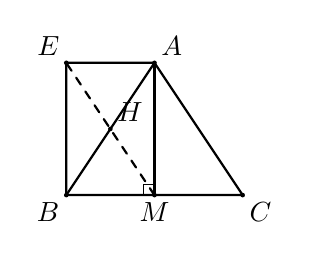
\begin{tikzpicture}[scale=0.70, >=stealth, line join=round, line cap=round]
  \coordinate (B) at (-1.6, 0);
  \coordinate (C) at (1.6, 0);
  \coordinate (M) at (0, 0);
  \coordinate (A) at (0, 2.4);
  \coordinate (H) at (-0.8, 1.2);
  \coordinate (E) at (-1.6, 2.4);
  \draw[thick] (C) -- (A) -- (E) -- (B) -- cycle;
  \draw[thick] (A) -- (M);
  \draw[thick] (A) -- (B);
  \draw[thick, dashed] (M) -- (E);
  \draw (0, 0.2) -- (-0.2, 0.2) -- (-0.2, 0);
  \fill (A) circle (1.2pt) node[above right=-1pt] {$A$};
  \fill (B) circle (1.2pt) node[below left=-1pt] {$B$};
  \fill (C) circle (1.2pt) node[below right=-1pt] {$C$};
  \fill (M) circle (1.2pt) node[below=-1pt] {$M$};
  \fill (H) circle (1.2pt) node[above right=-1pt] {$H$};
  \fill (E) circle (1.2pt) node[above left=-1pt] {$E$};
\end{tikzpicture}
\end{minipage}\par
\vspace{0.4mm}
\noindent\textit{Bài giải:}\dongkeHaiCot{11}
\\ \hline
\end{tabularx}

\vspace{1.4mm}

\noindent
\begin{tabularx}{\linewidth}{|X|}
\hline
\vspace{0.5mm}
\textbf{Câu 14 (0,5 điểm).} Tìm giá trị lớn nhất của biểu thức: $B = -x^2 + 8x + 2009$.\par
\vspace{0.4mm}
\noindent\textit{Bài giải:}\dongkeHaiCot{7}
\\ \hline
\end{tabularx}

\newpage
% =============================================================================
% ========================= TOAN 8 TUAN 09 BUOI 02 - MA DE 103 =================
% ========================= TRANG 1/2 ==========================================
% =============================================================================
\noindent
\begin{tabularx}{\linewidth}{|X|c|}
\hline
\textbf{PHIẾU KIỂM TRA ĐỊNH KỲ TOÁN 8 - TUẦN 09 - BUỔI 02} & \textbf{Mã đề: 103 - Trang 1/2} \\
\hline
\end{tabularx}

\vspace{1.2mm}

\noindent
\begin{tabularx}{\linewidth}{|p{3.2cm}|X|}
\hline
\centering\textbf{ĐIỂM SỐ} & \centering\textbf{LỜI NHẬN XÉT CỦA THẦY CÔ} \tabularnewline
\hline
\rule{0pt}{1.8cm} & \tabularnewline
\hline
\end{tabularx}

\vspace{1.4mm}
\noindent\textbf{Câu 1 (0,25 điểm).} Bậc của đơn thức $C = 4x^5 y z^2$ là: \shortans{8}\par\vspace{2.3mm}
\noindent\textbf{Câu 2 (0,25 điểm).} Bậc của đa thức $R = 3x^4 y - 4x^2 y^2 - 3x^4 y + x^2 y^2 + 7$ là: \shortans{4}\par\vspace{2.3mm}
\noindent\textbf{Câu 3 (0,25 điểm).} Giá trị của $P = 4x^2 y - 3xy$ tại $x=-1, y=2$ bằng: \shortans{14}\par\vspace{2.3mm}
\noindent\textbf{Câu 4 (0,25 điểm).} Cho khai triển $(x-6)(x+6) = x^2 - c$. Giá trị của $c$ là: \shortans{36}\par\vspace{2.3mm}
\noindent\textbf{Câu 5 (0,25 điểm).} Tính nhanh giá trị biểu thức $102^2 - 4 = $: \shortans{10\,400}\par\vspace{2.3mm}
\noindent\textbf{Câu 6 (0,25 điểm).} Phân tích đa thức thành bình phương: $x^2 + 12x + 36 = $: \shortans{(x + 6)^2}\par\vspace{2.3mm}
\noindent\textbf{Câu 7 (0,25 điểm).} Kết quả phép chia $(20x^3 y^3 - 15x^2 y^2) : (5x^2 y^2)$ là: \shortans{4xy - 3}\par\vspace{2.3mm}
\noindent\textbf{Câu 8 (0,25 điểm).} Hình thoi có chu vi $32\text{ cm}$. Độ dài mỗi cạnh của hình thoi là: \shortans{8\text{ cm}}\par\vspace{2.3mm}
\noindent\textbf{Câu 9 (0,25 điểm).} Hình thoi có một góc vuông là hình gì?: \shortans{Hình vuông}\par\vspace{2.3mm}
\noindent\textbf{Câu 10 (0,25 điểm).} Hình thoi có độ dài hai đường chéo là $8\text{ m}$ và $14\text{ m}$. Diện tích hình thoi là: \shortans{56\text{ m}^2}\par\vspace{2.3mm}
\vspace{0.2mm}
\noindent\textbf{Câu 11 (3,0 điểm). Thực hiện phép tính và phân tích đa thức thành nhân tử:}
\vspace{0.8mm}

\noindent
\begin{tabularx}{\linewidth}{|X|X|}
\hline
\oBaiTap[6]{a) (0,5 điểm)}{$4x(2x^2 - 3x + 4)$} & 
\oBaiTap[6]{b) (0,5 điểm)}{$(2x - 3)(x + 5) - 2x^2$} \\
\hline
\oBaiTap[6]{c) (0,5 điểm)}{$(x - 4)^2 + (x + 4)^2$} & 
\oBaiTap[6]{d) (0,5 điểm)}{$x^2 - xy + 5x - 5y$} \\
\hline
\oBaiTap[6]{e) (0,5 điểm)}{$x^2 - 16y^2 + 6x + 9$} & 
\oBaiTap[6]{f) (0,5 điểm)}{$x^2 - 6x + 8$} \\
\hline
\end{tabularx}

\newpage
% =============================================================================
% ========================= TOAN 8 TUAN 09 BUOI 02 - MA DE 103 =================
% ========================= TRANG 2/2 ==========================================
% =============================================================================
\noindent
\begin{tabularx}{\linewidth}{|X|c|}
\hline
\textbf{TOÁN 8 - TUẦN 09 - BUỔI 02} & \textbf{Mã đề: 103 - Trang 2/2} \\
\hline
\end{tabularx}

\vspace{1.4mm}

\noindent\textbf{Câu 12 (2,0 điểm). Tìm số thực $x$, biết:}
\vspace{0.8mm}

\noindent
\begin{tabularx}{\linewidth}{|X|X|}
\hline
\oBaiTap[5]{a) (0,5 điểm)}{$5x(x - 2) - 5x^2 = -40$} & 
\oBaiTap[5]{b) (0,5 điểm)}{$x(x - 5) + 3(x - 5) = 0$} \\
\hline
\oBaiTap[5]{c) (0,5 điểm)}{$(x - 4)^2 - 49 = 0$} & 
\oBaiTap[5]{d) (0,5 điểm)}{$(2x - 3)^2 = 25$} \\
\hline
\end{tabularx}

\vspace{1.4mm}

\noindent
\begin{tabularx}{\linewidth}{|X|}
\hline
\vspace{0.5mm}
\begin{minipage}[t]{0.64\linewidth}
\vspace{0pt}
\textbf{Câu 13 (2,0 điểm).} Cho tam giác $MNP$ cân tại $M$, đường trung tuyến $MI$. Gọi $K$ là trung điểm của $MP$. Lấy điểm $E$ đối xứng với $I$ qua $K$.\par\vspace{0.4mm}
\textbf{a)} (1,0 điểm) Chứng minh tứ giác $MIPE$ là hình chữ nhật.\par\vspace{0.4mm}
\textbf{b)} (1,0 điểm) Chứng minh tứ giác $MNIE$ là hình bình hành. Suy ra $ME \parallel NP$ và $ME = IP$.
\end{minipage}\hfill
\begin{minipage}[t]{0.34\linewidth}
\vspace{0pt}\centering
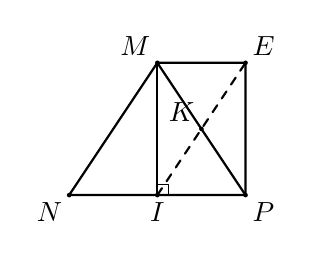
\begin{tikzpicture}[scale=0.70, >=stealth, line join=round, line cap=round]
  \coordinate (N) at (-1.6, 0);
  \coordinate (P) at (1.6, 0);
  \coordinate (I) at (0, 0);
  \coordinate (M) at (0, 2.4);
  \coordinate (K) at (0.8, 1.2);
  \coordinate (E) at (1.6, 2.4);
  \draw[thick] (N) -- (M) -- (E) -- (P) -- cycle;
  \draw[thick] (M) -- (I);
  \draw[thick] (M) -- (P);
  \draw[thick, dashed] (I) -- (E);
  \draw (0, 0.2) -- (0.2, 0.2) -- (0.2, 0);
  \fill (M) circle (1.2pt) node[above left=-1pt] {$M$};
  \fill (N) circle (1.2pt) node[below left=-1pt] {$N$};
  \fill (P) circle (1.2pt) node[below right=-1pt] {$P$};
  \fill (I) circle (1.2pt) node[below=-1pt] {$I$};
  \fill (K) circle (1.2pt) node[above left=-1pt] {$K$};
  \fill (E) circle (1.2pt) node[above right=-1pt] {$E$};
\end{tikzpicture}
\end{minipage}\par
\vspace{0.4mm}
\noindent\textit{Bài giải:}\dongkeHaiCot{11}
\\ \hline
\end{tabularx}

\vspace{1.4mm}

\noindent
\begin{tabularx}{\linewidth}{|X|}
\hline
\vspace{0.5mm}
\textbf{Câu 14 (0,5 điểm).} Tìm giá trị lớn nhất của biểu thức: $B = -x^2 + 4x + 2022$.\par
\vspace{0.4mm}
\noindent\textit{Bài giải:}\dongkeHaiCot{7}
\\ \hline
\end{tabularx}

\newpage
% =============================================================================
% ========================= TOAN 8 TUAN 09 BUOI 02 - MA DE 104 =================
% ========================= TRANG 1/2 ==========================================
% =============================================================================
\noindent
\begin{tabularx}{\linewidth}{|X|c|}
\hline
\textbf{PHIẾU KIỂM TRA ĐỊNH KỲ TOÁN 8 - TUẦN 09 - BUỔI 02} & \textbf{Mã đề: 104 - Trang 1/2} \\
\hline
\end{tabularx}

\vspace{1.2mm}

\noindent
\begin{tabularx}{\linewidth}{|p{3.2cm}|X|}
\hline
\centering\textbf{ĐIỂM SỐ} & \centering\textbf{LỜI NHẬN XÉT CỦA THẦY CÔ} \tabularnewline
\hline
\rule{0pt}{1.8cm} & \tabularnewline
\hline
\end{tabularx}

\vspace{1.4mm}
\noindent\textbf{Câu 1 (0,25 điểm).} Bậc của đơn thức $D = -6x^2 y^4 z^3$ là: \shortans{9}\par\vspace{2.3mm}
\noindent\textbf{Câu 2 (0,25 điểm).} Bậc của đa thức $S = 6x y^3 - 5x^2 + 9 - 6x y^3 + 2x^2$ là: \shortans{2}\par\vspace{2.3mm}
\noindent\textbf{Câu 3 (0,25 điểm).} Giá trị của $Q = 2x^2 y - 5xy$ tại $x=-1, y=3$ bằng: \shortans{21}\par\vspace{2.3mm}
\noindent\textbf{Câu 4 (0,25 điểm).} Cho khai triển $(x-7)(x+7) = x^2 - d$. Giá trị của $d$ là: \shortans{49}\par\vspace{2.3mm}
\noindent\textbf{Câu 5 (0,25 điểm).} Tính nhanh giá trị biểu thức $99^2 - 1 = $: \shortans{9\,800}\par\vspace{2.3mm}
\noindent\textbf{Câu 6 (0,25 điểm).} Phân tích đa thức thành bình phương: $x^2 + 14x + 49 = $: \shortans{(x + 7)^2}\par\vspace{2.3mm}
\noindent\textbf{Câu 7 (0,25 điểm).} Kết quả phép chia $(14x^4 y^2 - 7x^2 y) : (7x^2 y)$ là: \shortans{2x^2 y - 1}\par\vspace{2.3mm}
\noindent\textbf{Câu 8 (0,25 điểm).} Hình thoi có chu vi $48\text{ cm}$. Độ dài mỗi cạnh của hình thoi là: \shortans{12\text{ cm}}\par\vspace{2.3mm}
\noindent\textbf{Câu 9 (0,25 điểm).} Hình thoi có hai đường chéo bằng nhau là hình gì?: \shortans{Hình vuông}\par\vspace{2.3mm}
\noindent\textbf{Câu 10 (0,25 điểm).} Hình thoi có độ dài hai đường chéo là $12\text{ m}$ và $16\text{ m}$. Diện tích hình thoi là: \shortans{96\text{ m}^2}\par\vspace{2.3mm}
\vspace{0.2mm}
\noindent\textbf{Câu 11 (3,0 điểm). Thực hiện phép tính và phân tích đa thức thành nhân tử:}
\vspace{0.8mm}

\noindent
\begin{tabularx}{\linewidth}{|X|X|}
\hline
\oBaiTap[6]{a) (0,5 điểm)}{$5x(2x^2 - 4x + 3)$} & 
\oBaiTap[6]{b) (0,5 điểm)}{$(3x - 2)(x + 4) - 3x^2$} \\
\hline
\oBaiTap[6]{c) (0,5 điểm)}{$(2x - 1)^2 + (2x + 1)^2$} & 
\oBaiTap[6]{d) (0,5 điểm)}{$x^2 - xy + 2x - 2y$} \\
\hline
\oBaiTap[6]{e) (0,5 điểm)}{$x^2 - 25y^2 + 8x + 16$} & 
\oBaiTap[6]{f) (0,5 điểm)}{$x^2 - 8x + 15$} \\
\hline
\end{tabularx}

\newpage
% =============================================================================
% ========================= TOAN 8 TUAN 09 BUOI 02 - MA DE 104 =================
% ========================= TRANG 2/2 ==========================================
% =============================================================================
\noindent
\begin{tabularx}{\linewidth}{|X|c|}
\hline
\textbf{TOÁN 8 - TUẦN 09 - BUỔI 02} & \textbf{Mã đề: 104 - Trang 2/2} \\
\hline
\end{tabularx}

\vspace{1.4mm}

\noindent\textbf{Câu 12 (2,0 điểm). Tìm số thực $x$, biết:}
\vspace{0.8mm}

\noindent
\begin{tabularx}{\linewidth}{|X|X|}
\hline
\oBaiTap[5]{a) (0,5 điểm)}{$2x(x - 5) - 2x^2 = -30$} & 
\oBaiTap[5]{b) (0,5 điểm)}{$x(x - 8) + 2(x - 8) = 0$} \\
\hline
\oBaiTap[5]{c) (0,5 điểm)}{$(x - 1)^2 - 64 = 0$} & 
\oBaiTap[5]{d) (0,5 điểm)}{$(3x + 1)^2 = 64$} \\
\hline
\end{tabularx}

\vspace{1.4mm}

\noindent
\begin{tabularx}{\linewidth}{|X|}
\hline
\vspace{0.5mm}
\begin{minipage}[t]{0.64\linewidth}
\vspace{0pt}
\textbf{Câu 13 (2,0 điểm).} Cho tam giác $DEF$ cân tại $D$, đường trung tuyến $DI$. Gọi $H$ là trung điểm của $DE$. Lấy điểm $G$ đối xứng với $I$ qua $H$.\par\vspace{0.4mm}
\textbf{a)} (1,0 điểm) Chứng minh tứ giác $DIEG$ là hình chữ nhật.\par\vspace{0.4mm}
\textbf{b)} (1,0 điểm) Chứng minh tứ giác $DFIG$ là hình bình hành. Suy ra $DG \parallel EF$ và $DG = IE$.
\end{minipage}\hfill
\begin{minipage}[t]{0.34\linewidth}
\vspace{0pt}\centering
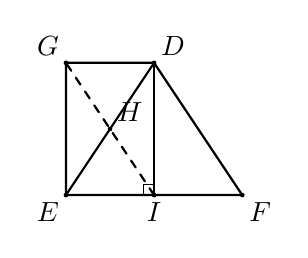
\begin{tikzpicture}[scale=0.70, >=stealth, line join=round, line cap=round]
  \coordinate (E) at (-1.6, 0);
  \coordinate (F) at (1.6, 0);
  \coordinate (I) at (0, 0);
  \coordinate (D) at (0, 2.4);
  \coordinate (H) at (-0.8, 1.2);
  \coordinate (G) at (-1.6, 2.4);
  \draw[thick] (F) -- (D) -- (G) -- (E) -- cycle;
  \draw[thick] (D) -- (I);
  \draw[thick] (D) -- (E);
  \draw[thick, dashed] (I) -- (G);
  \draw (0, 0.2) -- (-0.2, 0.2) -- (-0.2, 0);
  \fill (D) circle (1.2pt) node[above right=-1pt] {$D$};
  \fill (E) circle (1.2pt) node[below left=-1pt] {$E$};
  \fill (F) circle (1.2pt) node[below right=-1pt] {$F$};
  \fill (I) circle (1.2pt) node[below=-1pt] {$I$};
  \fill (H) circle (1.2pt) node[above right=-1pt] {$H$};
  \fill (G) circle (1.2pt) node[above left=-1pt] {$G$};
\end{tikzpicture}
\end{minipage}\par
\vspace{0.4mm}
\noindent\textit{Bài giải:}\dongkeHaiCot{11}
\\ \hline
\end{tabularx}

\vspace{1.4mm}

\noindent
\begin{tabularx}{\linewidth}{|X|}
\hline
\vspace{0.5mm}
\textbf{Câu 14 (0,5 điểm).} Tìm giá trị lớn nhất của biểu thức: $B = -x^2 + 10x + 2002$.\par
\vspace{0.4mm}
\noindent\textit{Bài giải:}\dongkeHaiCot{7}
\\ \hline
\end{tabularx}
\end{document}
